% Two comparisons of the same cohort at the same rounded kappa,
% and the tables their printed figures determine.
% Numbers: results/goyal_all_pairs.json (Goyal et al. 2025, Table 3 / Figure 2).
% House vocabulary: HOUSE_STYLE/docs/viz.md. Compile: pdflatex fig_two_cases.tex
\documentclass[tikz,border=6pt]{standalone}
\usepackage{amsmath,amssymb}
\usetikzlibrary{arrows.meta,positioning}

\definecolor{boxblue}{HTML}{DBEAFE}  \definecolor{bordblue}{HTML}{3B82F6}
\definecolor{boxred}{HTML}{FEE2E2}   \definecolor{bordred}{HTML}{DC2626}
\definecolor{boxgreen}{HTML}{D1FAE5} \definecolor{bordgreen}{HTML}{059669}
\definecolor{anncolor}{HTML}{6B7280} \definecolor{ink}{HTML}{1B2A41}

\begin{document}
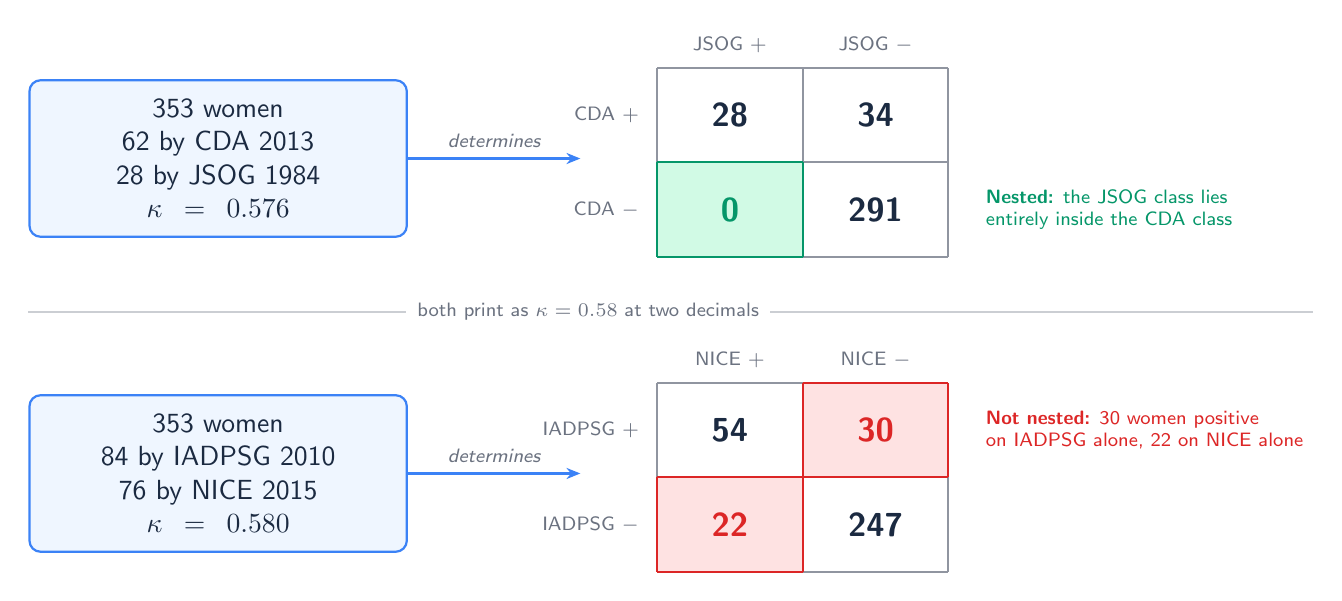
\begin{tikzpicture}[
    font=\sffamily,
    printbox/.style={rectangle, rounded corners=4pt, text centered, line width=0.8pt,
                     inner sep=7pt, draw=bordblue, fill=boxblue!45, text width=4.3cm,
                     text=ink},
    % Cells carry fill and text only. Every rule is drawn once, below, because a
    % cell border stroked by both of its neighbours renders heavier than an outer
    % edge stroked once.
    % outer sep=0pt puts the anchors on the box itself; with the default half-line-width
    % offset, a cell's north anchor sits above its neighbour's south and the rules between
    % them are drawn a fraction of a point apart.
    cell/.style={rectangle, minimum width=1.85cm, minimum height=1.2cm, text centered,
                 font=\sffamily\bfseries\large, draw=none, fill=white, text=ink,
                 outer sep=0pt},
    keycell/.style={cell, fill=boxred, text=bordred},
    nestcell/.style={cell, fill=boxgreen, text=bordgreen},
    rule/.style={line width=0.7pt, color=anncolor!75},
    keyrule/.style={line width=0.7pt, color=bordred},
    nestrule/.style={line width=0.7pt, color=bordgreen},
    hdr/.style={font=\sffamily\scriptsize, color=anncolor},
    ann/.style={font=\sffamily\scriptsize, color=anncolor, align=left},
    onarrow/.style={font=\sffamily\scriptsize\itshape, color=anncolor},
    arr/.style={-{Stealth[length=5pt,width=4pt]}, line width=1.1pt, color=bordblue},
]

%% ---- upper case: one class inside the other --------------------------------
\node[printbox] (pA) at (0,2.5)
    {353 women\\ 62 by CDA 2013\\ 28 by JSOG 1984\\ $\kappa = 0.576$};
\draw[arr] (pA.east) -- node[onarrow, above] {determines} (4.6,2.5);

\node[cell]    (a11) at (6.5,3.05) {28};
\node[cell]    (a10) at (8.35,3.05) {34};
\node[cell]    (a00) at (8.35,1.85) {291};
\node[nestcell] (a01) at (6.5,1.85) {0};
% twelve rules, each drawn once: the four around the nested cell in green
\draw[rule] (a11.north west) -- (a11.north east);  \draw[rule] (a10.north west) -- (a10.north east);
\draw[rule] (a10.south west) -- (a10.south east);  \draw[rule] (a00.south west) -- (a00.south east);
\draw[rule] (a11.north west) -- (a11.south west);  \draw[rule] (a11.north east) -- (a11.south east);
\draw[rule] (a10.north east) -- (a10.south east);  \draw[rule] (a00.north east) -- (a00.south east);
\draw[nestrule] (a01.north west) -- (a01.north east);
\draw[nestrule] (a01.south west) -- (a01.south east);
\draw[nestrule] (a01.north west) -- (a01.south west);
\draw[nestrule] (a01.north east) -- (a01.south east);
\node[hdr, above=2pt of a11] {JSOG $+$};   \node[hdr, above=2pt of a10] {JSOG $-$};
\node[hdr, left=3pt of a11] {CDA $+$};     \node[hdr, left=3pt of a01] {CDA $-$};
\node[ann, right=10pt of a00] (nA)
    {\textcolor{bordgreen}{\bfseries Nested:} \textcolor{bordgreen}{the JSOG class lies}\\
     \textcolor{bordgreen}{entirely inside the CDA class}};

%% ---- lower case: each identifies women the other does not -------------------
\node[printbox] (pB) at (0,-1.5)
    {353 women\\ 84 by IADPSG 2010\\ 76 by NICE 2015\\ $\kappa = 0.580$};
\draw[arr] (pB.east) -- node[onarrow, above] {determines} (4.6,-1.5);

\node[cell]    (b11) at (6.5,-0.95) {54};
\node[cell]    (b00) at (8.35,-2.15) {247};
\node[keycell] (b10) at (8.35,-0.95) {30};
\node[keycell] (b01) at (6.5,-2.15) {22};
% the eight around the two cells outside the nesting in red
\draw[rule] (b11.north west) -- (b11.north east);  \draw[rule] (b11.north west) -- (b11.south west);
\draw[rule] (b00.south west) -- (b00.south east);  \draw[rule] (b00.north east) -- (b00.south east);
\draw[keyrule] (b10.north west) -- (b10.north east);
\draw[keyrule] (b10.south west) -- (b10.south east);
\draw[keyrule] (b10.north west) -- (b10.south west);
\draw[keyrule] (b10.north east) -- (b10.south east);
\draw[keyrule] (b01.north west) -- (b01.north east);
\draw[keyrule] (b01.south west) -- (b01.south east);
\draw[keyrule] (b01.north west) -- (b01.south west);
\draw[keyrule] (b01.north east) -- (b01.south east);
\node[hdr, above=2pt of b11] {NICE $+$};    \node[hdr, above=2pt of b10] {NICE $-$};
\node[hdr, left=3pt of b11] {IADPSG $+$};   \node[hdr, left=3pt of b01] {IADPSG $-$};
\node[ann, right=10pt of b10] (nB)
    {\textcolor{bordred}{\bfseries Not nested:} \textcolor{bordred}{30 women positive}\\
     \textcolor{bordred}{on IADPSG alone, 22 on NICE alone}};

%% ---- divider ----------------------------------------------------------------
\coordinate (div) at (0,0.55);
\draw[anncolor!35, line width=0.5pt] (pA.west |- div) -- (nB.east |- div);
\node[ann, align=center, fill=white, inner sep=4pt] at (4.7,0.55)
    {both print as $\kappa = 0.58$ at two decimals};

\end{tikzpicture}
\end{document}
